\section{Die Welt der Preisvergleichsportale}
\label{sec:einleitung}

Der Fernhandel ist bereits seit Urzeiten ein wichtiger Bestandteil der Gesellschaft.
Durch die rasante Entwicklung des Internets und die steigende Anzahl der Onlinehändler vergrößert sich das
Produktangebot.
Heutzutage kann ein Käufer aus einer Vielzahl von Artikeln wählen und muss sich nicht, wie in der Urzeit, auf
einen Händler oder auf die lokale Verfügbarkeit beschränken.

\subsection{Der Onlinehandel von heute}
\label{subsec:onlinehandel-heute}

In den letzten Jahren hat der Onlinehandel sowohl an Bedeutung für die Unternehmen, als auch für die Kunden gewonnen.
Laut einer Statistik von Eurostat machte im Jahr 2017 der Onlinehandel 21\% des Gesamtumsatzes deutscher Unternehmen
aus und stellte somit einen nicht unerheblichen Anteil an der wirtschaftlichen Leistung
dar~\cite{statista:anteil-gesamtumsatz-europa}.
Aus einer weiteren Untersuchung geht hervor, dass 2017 zwei Drittel der Deutschen regelmäßig online
einkauften~\cite{statista:anteil-online-kaeufer-europa}.

Diese Entwicklung bringt jedoch ein Problem mit sich: Mit der steigenden Auswahl an Produkten und vor allem Händlern
verliert ein potenzieller Käufer schnell die Übersicht.
Preisvergleichsportale versuchen deshalb die Markttransparenz wiederherzustellen.
Ein Käufer sollte sich sicher sein können, das für ihn günstigste Angebot zu finden.

Das Angebot der Vergleichsportale wird von den Internetnutzern gut aufgenommen, wie eine Messung von 2017 zeigt:
Für einen besseren Vergleich nutzen rund zwei Drittel der Online-Käufer die Möglichkeit, sich im Internet zum Produkt
oder zum Preis zu informieren~\cite{statista:internetnutzer-preisvergleich-deutschland,
statista:anteil-online-kaeufe-deutschland}.
In einem vom Nachrichtensender n-tv beauftragten Test\footnotemark hat das Deutsche Institut für Service-Qualität
mehrere Preissuchmaschinen unter dem Aspekt des günstigsten Preises, der Aktualität des Preises und dem
Nutzererlebnis verglichen.
\footnotetext{\url{https://disq.de/2014/20141004-Preissuchmaschinen.html}}
Im Ergebnis hat idealo.de in allen Kategorien den ersten Platz eingenommen, gefolgt von billiger.de und preis.de.
Es wurde jedoch bemängelt, dass selbst beim besten Preisvergleich nur für die Hälfte der Produkte das günstigste
Angebot angezeigt wurde.

\subsection{Das Preisvergleichsportal idealo}
\label{subsec:idealo}

Die Mission des Preisvergleichsportals idealo ist es, im Sinne der Kundenzufriedenheit den Vergleich stetig zu
verbessern.
Je mehr Angebote idealo vergleicht, desto sicherer kann sich der Kunde sein, tatsächlich das günstigste Angebot zu
finden.
Dazu schließt idealo Verträge mit mehreren Onlinehändlern ab.
Diese Händler verpflichten sich, Daten zu ihren Angeboten an idealo zu übermitteln und zu aktualisieren.
Für jeden vermittelten Kauf zahlen die Shops an idealo eine Provision.
Diese Provision basiert auf CPC (Kosten pro Klick) oder CPO (Kosten pro tatsächlicher Bestellung).

Wie bereits in Kapitel~\ref{subsec:onlinehandel-heute} erwähnt, zeigt idealo bereits für 50\% der Produkte den
günstigsten Preis.
Um auch zukünftig wettbewerbsfähig zu bleiben, arbeitet idealo daran, auch für die letzten 50\% der Produkte
immer das beste Angebot liefern zu können.
Dies erreicht idealo zum einen durch Vertragsabschlüsse mit weiteren Onlineshops und zum anderen durch die
Sicherstellung, dass tatsächlich alle Angebote eines Vertragspartners gelistet werden.

\subsection{Das Ziel des Bachelorprojektes}
\label{subsec:projektziel}

Das Projektziel bestand darin, eine Software zu entwerfen, welche eine automatisierte Bestandsanalyse für
gegebene Vertragspartner durchführt.
Mit Hilfe des resultierenden Berichtes soll es möglich sein, herauszufinden, welche Angebote des Onlinehändlers im
Produktkatalog von idealo fehlen.
Der Ergebnisbericht soll Informationen darüber enthalten, welche Produkte nicht vorhanden sind und zu welcher
Preisregion die Produkte gehören.
Durch diese Übersicht soll ein Mitarbeiter von idealo dazu befähigt werden, die Ursachen für das Fehlen der Angebote
herauszufinden.

Mitarbeiter von idealo vermuten, dass ein unbeabsichtigtes Fehlen von Produkten möglicherweise durch einen fehlerhaften
Importvorgang zu erklären sei.
Zudem könnte es sein, dass ein Händler aufgrund spezieller Vertragsbedingungen bewusst nicht alle
Produkte bei idealo führen möchte.

Für die Entwicklung dieser Softwarelösung hatten wir als fünfköpfiges Team neun Monate Zeit.
Zudem wurde uns ein Betreuer von idealo zur Seite gestellt, welcher die funktionalen Anforderungen an die
Software kommunizierte und als technischer Berater diente.
Er begleitete uns während des gesamten Entwicklungsprozesses und unterstützte uns bei Fragen bezüglich der
Systemarchitektur.

\subsection{Die Microservice-Architektur des Scout-Softwaresystems}
\label{subsec:microservice-architektur}

Wir haben uns dafür entschieden, das Gesamtsystem als Microservice-Architektur zu konzipieren.
Die Microservice-Architektur ermöglicht es logisch gekapselte Komponenten zu entwickeln, welche sich sehr gut
skalieren und erweitern lassen.
Eine ausführlichere Begründung für diese Architekturentscheidung kann in der Bachelorarbeit von Dmitrii
Zhamanakov nachgeschlagen werden~\cite{thesis:dmitrii}.
Für die Implementierung der Architektur haben wir die Programmiersprache Java gewählt und verwenden diese in
Kombination mit dem Spring-Framework\footnotemark.
\footnotetext{\url{https://spring.io/}}
Das entwickelte Gesamtsystem \textit{Scout} besteht aus drei zentralen Komponenten: dem Crawler, dem Parser und dem
Matcher.
In Abbildung~\ref{abb:datenfluss-grob} ist der Datenfluss zwischen den Komponenten dargestellt.

\begin{figure}[H]
    \centering
    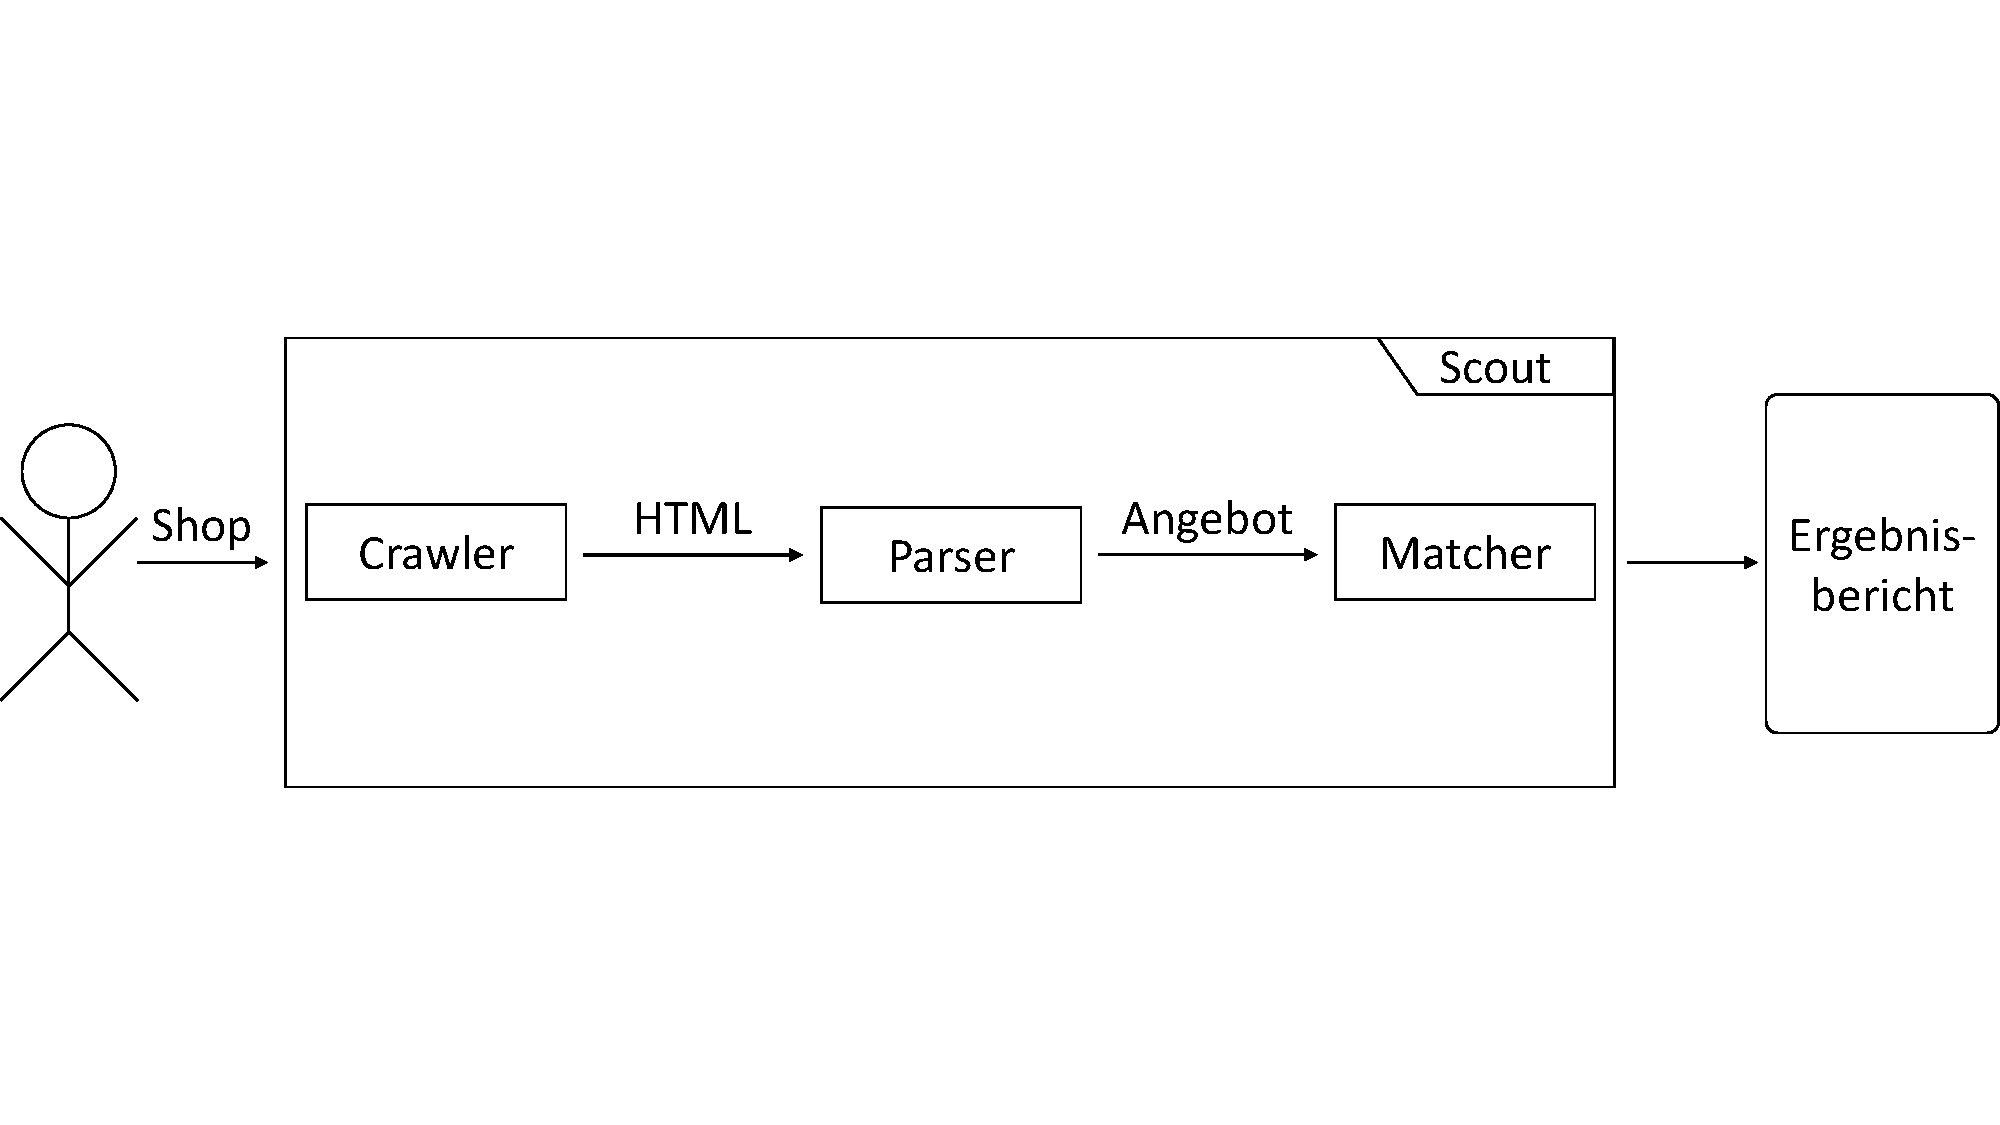
\includegraphics[width=\textwidth, trim=0 5.5cm 0 5.5cm, clip]{resources/Datenfluss-Gesamt-Grob.pdf}
    \caption{Datenfluss des Softwaresystems Scout}
    \label{abb:datenfluss-grob}
    \vspace{-0.25cm}
\end{figure}

Der \textit{Crawler} ist für das Herunterladen jeder einzelnen Seite eines durch den Nutzer spezifizierten Shops
verantwortlich.
Jonas Pohlmann hat sich im Projektverlauf intensiv mit verschiedenen Crawling-Frameworks auseinandergesetzt und diese
in seiner Bachelorarbeit verglichen~\cite{thesis:jonas}.

Die Funktionsweise der maschinenlernbasierten \textit{Matcher}-Komponente wird in der Bachelorarbeit von Tom
Schwarzburg näher beschrieben~\cite{thesis:tom}.
Der Matcher vergleicht die vom Parser gefundenen Angebote mit denen, die idealo bereits kennt und liefert
einen Bericht, in dem alle fehlenden Angebote aufgelistet werden.

Damit diese Komponente die geladenen Angebote mit dem Katalog von idealo vergleichen kann, muss das heruntergeladene
HTML-Dokument in ein Format gebracht werden, welches der Computer für den Vergleich nutzen kann.
Diesen Schritt erledigt der \textit{Parser}, welcher zwischen Crawler und Matcher agiert.
Der Fokus dieser Bachelorarbeit liegt in der Beschreibung der Funktionsweise und des Aufbaus des Parsers.